\documentclass[12pt,twocolumn]{article}
\usepackage[margin=0.5in]{geometry}
\def\inputGnumerictable{}
\usepackage[cmex10]{amsmath}
\usepackage{gensymb}
\usepackage{graphicx}
\usepackage{amsthm}
\usepackage{mathrsfs}
\usepackage{txfonts}
\usepackage{cite}
\usepackage{cases}
\usepackage{subfig}
\usepackage[breaklinks=true]{hyperref}
\usepackage{listings}
\usepackage[latin1]{inputenc}
    \usepackage{color}                                         
    \usepackage{array}                                         
    \usepackage{longtable}                       
    \usepackage{calc}                                            
    \usepackage{multirow}                                       
    \usepackage{hhline}                                           
    \usepackage{ifthen}                                           
    \usepackage{amssymb}
\providecommand{\pr}[1]{\ensuremath{\Pr\left(#1\right)}}
\newcommand*{\Comb}[2]{{}^{#1}C_{#2}}%
\title{
Probability Assignment
}
\author{GINNA SHREYANI}
\date{}
\providecommand{\pr}[1]{\ensuremath{\Pr\left(#1\right)}}
\providecommand{\brak}[1]{\ensuremath{\left(#1\right)}}
\providecommand{\cbrak}[1]{\ensuremath{\left\{#1\right\}}}
\providecommand{\lcbrak}[1]{\ensuremath{\left\{#1\right.}}
\providecommand{\rcbrak}[1]{\ensuremath{\left.#1\right\}}}

\begin{document}
\maketitle

\textbf{11.16.3.2}\\
A coin is tossed twice, what is the probability that atleast one tail occurs?\\
\subsection*{Solution}
By using binomial distribution we can find the probability of atleast one tail occurs hen a coin is tossed twice.\\
Here we are assuming when ever a tail shows up it is a success(1)\\
The Binomial Distribution: Let
\begin{align}
	Y &= \sum_{i=1}^n X_i
         \label{eq-1}
\end{align}
where n is the total number of times the coin is tossed. Then X has a binomial distribution. Then, for
\begin{align}
	&p_{X_i}(n){\stackrel{z}{\rightleftharpoons}}P_{X_i}(z),
     \label{eq-2}
\end{align}
yielding
\begin{align}
	P_{X_i}(Z) &= 1-p+pz^{-1}
	\label{eq-3}
\end{align}
Since $X_i$ are i.i.d.,
\begin{align}
	P_X(Z)&=(1-p+pz^{-1})^n\\
	&=\sum_{k=0}^n{\Comb{n}{k}p^{k}(1-p)^{n-k}}
\end{align}
\[
	p_X(k)=
	\begin{cases}
		\Comb{n}{k}p^{n-k}(1-p)^k,& \text{if } 0\leq k\leq n\\
		0,& \text{otherwise}
	\end{cases}
\]
As a result it is written as
\begin{align}
	\label{eq-6}
	p_X(k) &=\binom nk p^{k}(1-p)^{n-k}
\end{align}
The cumulative distribution function of X is defined as
\begin{align}
	F_X(r) &=\Pr(X\leq r) = \sum_{k=0}^r\binom nk p^{k}(1-p)^{n-k}
	\label{eq-7}
\end{align}
Therefore, we get the number of trails i.e., the number of times the coin is tossed and the probability of getting atleast one tail is sum of the probability of getting one tail and probability of getting two tails.
The probability of getting a tail when a coin is tossed is 0.5.
\begin{align}
	n &= 2\\
	r &= 1,2\\
	p &= 0.5
\end{align}
Therefore,
\begin{align}
	\Pr(Y\geq 1)&=\sum_{k=1}^2 \binom nk p^k(1-p)^{n-k}\\
	&=\binom 21(0.5)^1(1-0.5)^{2-1}+\binom 22 (0.5)^2(1-0.5)^{2-2}\\
	\Pr(Y\geq 1)&=0.5+0.25\\
	\Pr(Y\geq 1)&= 0.75
\end{align}
Therefore,the probability of getting atleast one tail whenthe coinis tossed twice is 0.75.\\
\begin{table}[h]
	%%%%%%%%%%%%%%%%%%%%%%%%%%%%%%%%%%%%%%%%%%%%%%%%%%%%%%%%%%%%%%%%%%%%%%
%%                                                                  %%
%%  This is the header of a LaTeX2e file exported from Gnumeric.    %%
%%                                                                  %%
%%  This file can be compiled as it stands or included in another   %%
%%  LaTeX document. The table is based on the longtable package so  %%
%%  the longtable options (headers, footers...) can be set in the   %%
%%  preamble section below (see PRAMBLE).                           %%
%%                                                                  %%
%%  To include the file in another, the following two lines must be %%
%%  in the including file:                                          %%
%%        \def\inputGnumericTable{}                                 %%
%%  at the beginning of the file and:                               %%
%%        \input{name-of-this-file.tex}                             %%
%%  where the table is to be placed. Note also that the including   %%
%%  file must use the following packages for the table to be        %%
%%  rendered correctly:                                             %%
%%    \usepackage[latin1]{inputenc}                                 %%
%%    \usepackage{color}                                            %%
%%    \usepackage{array}                                            %%
%%    \usepackage{longtable}                                        %%
%%    \usepackage{calc}                                             %%
%%    \usepackage{multirow}                                         %%
%%    \usepackage{hhline}                                           %%
%%    \usepackage{ifthen}                                           %%
%%  optionally (for landscape tables embedded in another document): %%
%%    \usepackage{lscape}                                           %%
%%                                                                  %%
%%%%%%%%%%%%%%%%%%%%%%%%%%%%%%%%%%%%%%%%%%%%%%%%%%%%%%%%%%%%%%%%%%%%%%



%%  This section checks if we are begin input into another file or  %%
%%  the file will be compiled alone. First use a macro taken from   %%
%%  the TeXbook ex 7.7 (suggestion of Han-Wen Nienhuys).            %%
\def\ifundefined#1{\expandafter\ifx\csname#1\endcsname\relax}


%%  Check for the \def token for inputed files. If it is not        %%
%%  defined, the file will be processed as a standalone and the     %%
%%  preamble will be used.                                          %%
\ifundefined{inputGnumericTable}

%%  We must be able to close or not the document at the end.        %%
	\def\gnumericTableEnd{\end{document}}


%%%%%%%%%%%%%%%%%%%%%%%%%%%%%%%%%%%%%%%%%%%%%%%%%%%%%%%%%%%%%%%%%%%%%%
%%                                                                  %%
%%  This is the PREAMBLE. Change these values to get the right      %%
%%  paper size and other niceties.                                  %%
%%                                                                  %%
%%%%%%%%%%%%%%%%%%%%%%%%%%%%%%%%%%%%%%%%%%%%%%%%%%%%%%%%%%%%%%%%%%%%%%

	\documentclass[12pt%
			  %,landscape%
                    ]{report}
       \usepackage[latin1]{inputenc}
       \usepackage{fullpage}
       \usepackage{color}
       \usepackage{array}
       \usepackage{longtable}
       \usepackage{calc}
       \usepackage{multirow}
       \usepackage{hhline}
       \usepackage{ifthen}

	\begin{document}


%%  End of the preamble for the standalone. The next section is for %%
%%  documents which are included into other LaTeX2e files.          %%
\else

%%  We are not a stand alone document. For a regular table, we will %%
%%  have no preamble and only define the closing to mean nothing.   %%
    \def\gnumericTableEnd{}

%%  If we want landscape mode in an embedded document, comment out  %%
%%  the line above and uncomment the two below. The table will      %%
%%  begin on a new page and run in landscape mode.                  %%
%       \def\gnumericTableEnd{\end{landscape}}
%       \begin{landscape}


%%  End of the else clause for this file being \input.              %%
\fi

%%%%%%%%%%%%%%%%%%%%%%%%%%%%%%%%%%%%%%%%%%%%%%%%%%%%%%%%%%%%%%%%%%%%%%
%%                                                                  %%
%%  The rest is the gnumeric table, except for the closing          %%
%%  statement. Changes below will alter the table's appearance.     %%
%%                                                                  %%
%%%%%%%%%%%%%%%%%%%%%%%%%%%%%%%%%%%%%%%%%%%%%%%%%%%%%%%%%%%%%%%%%%%%%%

\providecommand{\gnumericmathit}[1]{#1} 
%%  Uncomment the next line if you would like your numbers to be in %%
%%  italics if they are italizised in the gnumeric table.           %%
%\renewcommand{\gnumericmathit}[1]{\mathit{#1}}
\providecommand{\gnumericPB}[1]%
{\let\gnumericTemp=\\#1\let\\=\gnumericTemp\hspace{0pt}}
 \ifundefined{gnumericTableWidthDefined}
        \newlength{\gnumericTableWidth}
        \newlength{\gnumericTableWidthComplete}
        \newlength{\gnumericMultiRowLength}
        \global\def\gnumericTableWidthDefined{}
 \fi
%% The following setting protects this code from babel shorthands.  %%
 \ifthenelse{\isundefined{\languageshorthands}}{}{\languageshorthands{english}}
%%  The default table format retains the relative column widths of  %%
%%  gnumeric. They can easily be changed to c, r or l. In that case %%
%%  you may want to comment out the next line and uncomment the one %%
%%  thereafter                                                      %%
\providecommand\gnumbox{\makebox[0pt]}
%%\providecommand\gnumbox[1][]{\makebox}

%% to adjust positions in multirow situations                       %%
\setlength{\bigstrutjot}{\jot}
\setlength{\extrarowheight}{\doublerulesep}

%%  The \setlongtables command keeps column widths the same across  %%
%%  pages. Simply comment out next line for varying column widths.  %%
\setlongtables

\setlength\gnumericTableWidth{%
	78pt+%
	53pt+%
	50pt+%
	50pt+%
0pt}
\def\gumericNumCols{4}
\setlength\gnumericTableWidthComplete{\gnumericTableWidth+%
         \tabcolsep*\gumericNumCols*2+\arrayrulewidth*\gumericNumCols}
\ifthenelse{\lengthtest{\gnumericTableWidthComplete > \linewidth}}%
         {\def\gnumericScale{1*\ratio{\linewidth-%
                        \tabcolsep*\gumericNumCols*2-%
                        \arrayrulewidth*\gumericNumCols}%
{\gnumericTableWidth}}}%
{\def\gnumericScale{1}}

%%%%%%%%%%%%%%%%%%%%%%%%%%%%%%%%%%%%%%%%%%%%%%%%%%%%%%%%%%%%%%%%%%%%%%
%%                                                                  %%
%% The following are the widths of the various columns. We are      %%
%% defining them here because then they are easier to change.       %%
%% Depending on the cell formats we may use them more than once.    %%
%%                                                                  %%
%%%%%%%%%%%%%%%%%%%%%%%%%%%%%%%%%%%%%%%%%%%%%%%%%%%%%%%%%%%%%%%%%%%%%%

\ifthenelse{\isundefined{\gnumericColA}}{\newlength{\gnumericColA}}{}\settowidth{\gnumericColA}{\begin{tabular}{@{}p{78pt*\gnumericScale}@{}}x\end{tabular}}
\ifthenelse{\isundefined{\gnumericColB}}{\newlength{\gnumericColB}}{}\settowidth{\gnumericColB}{\begin{tabular}{@{}p{53pt*\gnumericScale}@{}}x\end{tabular}}
\ifthenelse{\isundefined{\gnumericColC}}{\newlength{\gnumericColC}}{}\settowidth{\gnumericColC}{\begin{tabular}{@{}p{50pt*\gnumericScale}@{}}x\end{tabular}}
\ifthenelse{\isundefined{\gnumericColD}}{\newlength{\gnumericColD}}{}\settowidth{\gnumericColD}{\begin{tabular}{@{}p{50pt*\gnumericScale}@{}}x\end{tabular}}

\begin{longtable}[c]{%
	b{\gnumericColA}%
	b{\gnumericColB}%
	b{\gnumericColC}%
	b{\gnumericColD}%
	}

%%%%%%%%%%%%%%%%%%%%%%%%%%%%%%%%%%%%%%%%%%%%%%%%%%%%%%%%%%%%%%%%%%%%%%
%%  The longtable options. (Caption, headers... see Goosens, p.124) %%
%	\caption{The Table Caption.}             \\	%
% \hline	% Across the top of the table.
%%  The rest of these options are table rows which are placed on    %%
%%  the first, last or every page. Use \multicolumn if you want.    %%

%%  Header for the first page.                                      %%
%	\multicolumn{4}{c}{The First Header} \\ \hline 
%	\multicolumn{1}{c}{colTag}	%Column 1
%	&\multicolumn{1}{c}{colTag}	%Column 2
%	&\multicolumn{1}{c}{colTag}	%Column 3
%	&\multicolumn{1}{c}{colTag}	\\ \hline %Last column
%	\endfirsthead

%%  The running header definition.                                  %%
%	\hline
%	\multicolumn{4}{l}{\ldots\small\slshape continued} \\ \hline
%	\multicolumn{1}{c}{colTag}	%Column 1
%	&\multicolumn{1}{c}{colTag}	%Column 2
%	&\multicolumn{1}{c}{colTag}	%Column 3
%	&\multicolumn{1}{c}{colTag}	\\ \hline %Last column
%	\endhead

%%  The running footer definition.                                  %%
%	\hline
%	\multicolumn{4}{r}{\small\slshape continued\ldots} \\
%	\endfoot

%%  The ending footer definition.                                   %%
%	\multicolumn{4}{c}{That's all folks} \\ \hline 
%	\endlastfoot
%%%%%%%%%%%%%%%%%%%%%%%%%%%%%%%%%%%%%%%%%%%%%%%%%%%%%%%%%%%%%%%%%%%%%%

\hhline{|-|-|-|-}
	 \multicolumn{1}{|p{\gnumericColA}|}%
	{\gnumericPB{\raggedright}\gnumbox[l]{\textbf{x(tails)}}}
	&\multicolumn{1}{p{\gnumericColB}|}%
	{\gnumericPB{\raggedleft}\gnumbox[r]{\textbf{0}}}
	&\multicolumn{1}{p{\gnumericColC}|}%
	{\gnumericPB{\raggedleft}\gnumbox[r]{\textbf{1}}}
	&\multicolumn{1}{p{\gnumericColD}|}%
	{\gnumericPB{\raggedleft}\gnumbox[r]{\textbf{2}}}
\\
\hhline{|----|}
	 \multicolumn{1}{|p{\gnumericColA}|}%
	{\gnumericPB{\raggedright}\gnumbox[l]{\textbf{P(X=x)}}}
	&\multicolumn{1}{p{\gnumericColB}|}%
	{\gnumericPB{\raggedleft}\gnumbox[r]{0.25}}
	&\multicolumn{1}{p{\gnumericColC}|}%
	{\gnumericPB{\raggedleft}\gnumbox[r]{0.5}}
	&\multicolumn{1}{p{\gnumericColD}|}%
	{\gnumericPB{\raggedleft}\gnumbox[r]{0.25}}
\\
\hhline{|----|}
	 \multicolumn{1}{|p{\gnumericColA}|}%
	{\gnumericPB{\raggedright}\gnumbox[l]{\textbf{P(X$>$=x)}}}
	&\multicolumn{1}{p{\gnumericColB}|}%
	{\gnumericPB{\raggedleft}\gnumbox[r]{1}}
	&\multicolumn{1}{p{\gnumericColC}|}%
	{\gnumericPB{\raggedleft}\gnumbox[r]{0.75}}
	&\multicolumn{1}{p{\gnumericColD}|}%
	{\gnumericPB{\raggedleft}\gnumbox[r]{0.25}}
\\
\hhline{|-|-|-|-|}
\end{longtable}

\ifthenelse{\isundefined{\languageshorthands}}{}{\languageshorthands{\languagename}}
\gnumericTableEnd

\end{table}

\begin{figure}[h]
    \centering
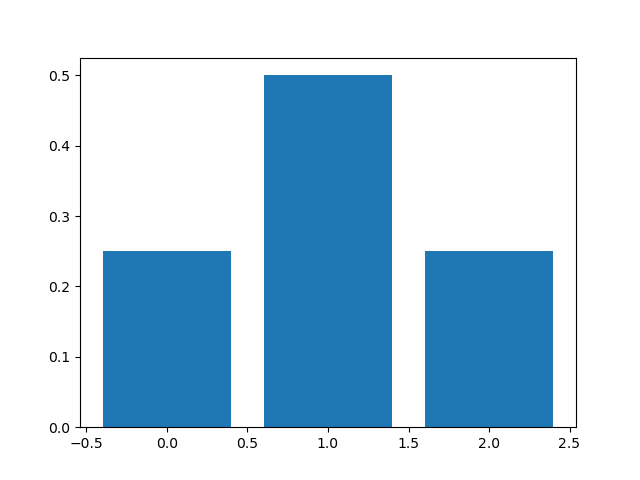
\includegraphics[width=\columnwidth]{fig/11.16.3.2.png}
\end{figure}
This is the code: \href{https://github.com/ShreyaniReddy/IITH-FWC/blob/main/probability/11.16.3.2/codes/11.16.3.2.py}{Code}
\end{document}
